%%%%%%%%%%%%%%%%%%%%%%%%%%%%%%%%%%%%%%%%%
% Beamer Presentation
% LaTeX Template
% Version 1.0 (10/11/12)
%
% This template has been downloaded from:
% http://www.LaTeXTemplates.com
%
% License:
% CC BY-NC-SA 3.0 (http://creativecommons.org/licenses/by-nc-sa/3.0/)
%
%%%%%%%%%%%%%%%%%%%%%%%%%%%%%%%%%%%%%%%%%

%----------------------------------------------------------------------------------------
%	PACKAGES AND THEMES
%----------------------------------------------------------------------------------------

\documentclass{beamer}

\mode<presentation> {

% The Beamer class comes with a number of default slide themes
% which change the colors and layouts of slides. Below this is a list
% of all the themes, uncomment each in turn to see what they look like.

%\usetheme{default}
%\usetheme{AnnArbor}
%\usetheme{Antibes}
%\usetheme{Bergen}
%\usetheme{Berkeley}
%\usetheme{Berlin}
%\usetheme{Boadilla}
%\usetheme{CambridgeUS}
%\usetheme{Copenhagen}
%\usetheme{Darmstadt}
%\usetheme{Dresden}
%\usetheme{Frankfurt}
%\usetheme{Goettingen}
%\usetheme{Hannover}
%\usetheme{Ilmenau}
%\usetheme{JuanLesPins}
%\usetheme{Luebeck}
\usetheme{Madrid}
%\usetheme{Malmoe}
%\usetheme{Marburg}
%\usetheme{Montpellier}
%\usetheme{PaloAlto}
%\usetheme{Pittsburgh}
%\usetheme{Rochester}
%\usetheme{Singapore}
%\usetheme{Szeged}
%\usetheme{Warsaw}

% As well as themes, the Beamer class has a number of color themes
% for any slide theme. Uncomment each of these in turn to see how it
% changes the colors of your current slide theme.

%\usecolortheme{albatross}
%\usecolortheme{beaver}
%\usecolortheme{beetle}
%\usecolortheme{crane}
%\usecolortheme{dolphin}
%\usecolortheme{dove}
%\usecolortheme{fly}
%\usecolortheme{lily}
%\usecolortheme{orchid}
%\usecolortheme{rose}
%\usecolortheme{seagull}
%\usecolortheme{seahorse}
%\usecolortheme{whale}
%\usecolortheme{wolverine}

%\setbeamertemplate{footline} % To remove the footer line in all slides uncomment this line
%\setbeamertemplate{footline}[page number] % To replace the footer line in all slides with a simple slide count uncomment this line

%\setbeamertemplate{navigation symbols}{} % To remove the navigation symbols from the bottom of all slides uncomment this line
}

\usepackage{graphicx} % Allows including images
\usepackage{booktabs} % Allows the use of \toprule, \midrule and \bottomrule in tables
\usepackage{listings}
\usepackage{amsmath}
\usepackage{algpseudocode,algorithm,algorithmicx}

\lstdefinestyle{custom}{
  breaklines=true,
  frame=L,
  xleftmargin=\parindent,
  language=Java,
  showstringspaces=false,
  basicstyle=\footnotesize\ttfamily,
  keywordstyle=\ttfamily\bfseries\color{green!40!black},
  commentstyle=\ttfamily\itshape\color{gray!40!black},
  identifierstyle=\color{blue},
  stringstyle=\color{orange},
  tabsize = 2
}

%----------------------------------------------------------------------------------------
%	TITLE PAGE
%----------------------------------------------------------------------------------------

\title[Hashing]{Hashing} % The short title appears at the bottom of every slide, the full title is only on the title page

\author{Jonathan Windle} % Your name
\institute[UEA] % Your institution as it will appear on the bottom of every slide, may be shorthand to save space
{
University of East Anglia \\ % Your institution for the title page
\medskip
\textit{J.Windle@uea.ac.uk} % Your email address
}
\date{\today} % Date, can be changed to a custom date

\begin{document}

\begin{frame}
\titlepage % Print the title page as the first slide
\end{frame}

\begin{frame}[allowframebreaks]
\frametitle{Overview} % Table of contents slide, comment this block out to remove it
\tableofcontents % Throughout your presentation, if you choose to use \section{} and \subsection{} commands, these will automatically be printed on this slide as an overview of your presentation
\end{frame} 

%------------------------------------------------------------------
\section{Intro}
\begin{frame}
\frametitle{Intro}
\small
\begin{itemize}
\item Technique for performing insertions,deletions and finds in a dictionary in {\color{green}constant average time}.
\item \textbf{Hash table:}
\begin{itemize}
\small
\item An array, $T$ of some fixed size is  used to store the keys.
\item \texttt{size} referres to the size of $T$.
\item $S = \{0,1,...,size -1\}$
\end{itemize}
\item \textbf{Hashing function:}
\begin{itemize}
\small
\item $h: K \rightarrow S.$
\item Suppose $K$ is the set of 6 digit non-negative integers, then a possible (but poor) choce for $h$ is:\\
\center
$h(k)=k(mod 1000)$
\end{itemize}
\item \textbf{Collisions:}
\begin{itemize}
\small
\item A collision occurs when two keys hash to the same location in the hash table:\\
$h(k) = h(k').$\\
\item Want to choose the hash function to minimise the chance of collisions.
\item Need to decide how to handle collisions when they do occur.
\end{itemize}
\end{itemize}
\end{frame}
%----------------------------------------------------------------
\section{Choosing Hash Function}
\begin{frame}
\frametitle{Choosing a Hash Function}
\begin{itemize}
\item A good hash function maps keys {\color{red}uniformly} and {\color{green}randomly} into the full range of possible locations.
\item A good hash function should depend on all of the charactersf the characters in a key, but this is not a sufficient condition for a good hash function.
\item Must not just depend on all of the characters in a key but must also distribute keys evenly over the table.
\item The built in Java function \texttt{hashCode} returns an integer based on the objects {\color{blue}reference} unless the object is a string then it is based on the string itself.
\item The Java class \texttt{HashTable} can be used with keys of any user-defined data type provided an instance method \texttt{hashCode} is defined.
\end{itemize}
\end{frame}
%----------------------------------------------------------------
\section{Resolving Collisions}
\begin{frame}
\frametitle{Resolving Collisions}
\begin{itemize}
\item Use some other location that is open in the table:
\begin{itemize}
\item {\color{red} Open addressing}
\end{itemize}
\item Change the structure of the hash table so that each location can correspond to more than one value:
\begin{itemize}
\item {\color{green}Chaining}.
\item {\color{purple}Buckets}.
\end{itemize}
\end{itemize}
\end{frame}
%----------------------------------------------------------------
\subsection{Chaining/Buckets}
\begin{frame}
\frametitle{Chaining/Buckets}
\begin{itemize}
\item Chaining:
\begin{itemize}
\item For each location $T$, keep a {\color{red} list} of allthe keys hashed to that location.
\item Each entry in $T$ is thus a reference to a linked list of keys.
\item To form a search, just hash to find the list and then perform the appropriate operation.
\end{itemize}
\item Buckets:
\begin{itemize}
\item Each location in the hash table is a bucket.
\item A fixed number, $b$ of locations to store the keys.
\item Total space available is thus:\\
$size \times b$
\end{itemize}
\end{itemize}
\end{frame}
%----------------------------------------------------------------
\subsection{Open Addressing}
\begin{frame}
\frametitle{Open Addressing}
\begin{itemize}
\item If a collision occurs, alternative cells in $T$ are tried until an empty cell is found.
\item Locating an open loaction in te hash table is called {\color{green}probing} 
\item May be necessary to try more than one alternqative location.
\item The locations examined when a new key is inserted is called a {\color{purple}probe sequence}.
\item Let $\langle S_j^k\rangle$ denote the probe sequence then:\\
$s_0^k = h(k)$\\
$s_j^k = (s^k_{j-1} + p(j,k))\%size, \quad j \geq 1$.\\
\item Where $p(j,k)$ is called a {\color{red}probe increment}.
\item In the simplist scheme the probe increment is independant of both $j$ and $k$. i.e. it is a constant $p$ in particular {\color{magenta}linear probing}, $p=1$.
\end{itemize}
\end{frame}
%----------------------------------------------------------------
\subsection{Linear Probing}
\begin{frame}
\frametitle{Linear Probing}
\begin{itemize}
\item If $T[h(k)]$ is occupied, try successive locations in $T$ with wrap-around.
\item Retrieval must be able to follow the same path used on insertion.
\item Care must be taken over deletion:
\begin{itemize}
\item When searching for the key, if an empty location is encountered before the key is found, this implies that the key is not present in $T$.
\item Only flag a location for deletion in a delete operation, otherwise a subsequent search might reach an incorrect conclusion.
\end{itemize}
\item When inserting should first check that the given key is not already present in the table:
\begin{itemize}
\item If not, {\color{red}probe sequence} ends and is added into the empty location.
\item May encounter flagged locations before hitting the empty location.
\item If we record the position of the first flagged location encountered we can store the entry in that location.
\end{itemize}
\item Been shown that provided load factor is 0.5 (half full table), only 2.5 probes are required onaverage for insertion and only 1.5 on average for a successful search.
\end{itemize}
\end{frame}
%------------------------------------------------------------------
\subsection{Clustering}
\begin{frame}
\frametitle{Clustering}
\begin{itemize}
\item Resolving collisions with linear probing leads to clusters of occupied locations.
\item Suppose when inserting we hash to a location $k$ in the table and we then have to go through a probe sequence of length $r$.
\item The next time we hash to location $k$ we need to go through a probe sequence of length $r+1$ at least.
\item Each addition to the table, increases the size of some cluster by 1 (at least - may also get merging of clusters).
\item Known as {\color{green}primary clustering}.
\end{itemize}
\end{frame}
%------------------------------------------------------------------
\defverbatim[colored]\qp{
\begin{lstlisting}[style = custom]
int i = h(k);
int j = 0;
while (T[i].key != emptyKey) {
	j++;
	i += 2*j - 1%T.size;
}
T[i].key = k;
T[i].data = d;
\end{lstlisting}
}
\subsection{Quadratic Probing}
\begin{frame}[allowframebreaks]
\frametitle{Quadratic Probing}
\begin{itemize}
\item Some schenes, the probe increment depends on the value of the index, $j$, in the probe sequence, but is still independant of $k$.
\item In quadratic probing, the probe sequence is given by:\\
\begin{center}
$s_j^k = (h(k)+j^2)\%size$\\
\end{center}
i.e.\\
\begin{center}
$s_0^k = h(k)$\\
$s^k_j = (s^k_{j-1} + 2j - 1)\%size, \quad j \geq 1,$\\
\end{center}
since\\
\begin{center}
$j^2 = (j-1)^2+2j-1$
\end{center}
\item The increment function for quadratic probing is $inc(j,k) = 2j-1$
\end{itemize}
\qp
\end{frame}
%-----------------------------------------------------------------
\subsubsection{Must be prime}
\begin{frame}
\frametitle{Must be prime}
\begin{itemize}
\item If size is not prime then there are only $p$ locations that can be generated as alternative loctions when a clash occurs.
\item However, if a size is a prime, and $T$ is at least half empty, a key can always be inserted.
\end{itemize}
\end{frame}
%-----------------------------------------------------------------
\subsubsection{Example}
\begin{frame}
\frametitle{Example}
\begin{itemize}
\item $h(k) = k\%13$
\item Insert 8,42,29,51,47,13,26 into table of size 13:\\
\end{itemize}
\begin{columns}[t]
\column{0.5\textwidth}
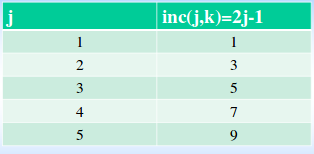
\includegraphics[scale=0.25]{j.png}\\
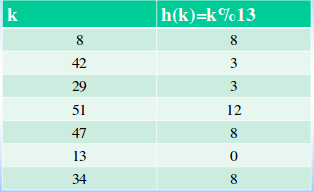
\includegraphics[scale=0.25]{k.png}\\
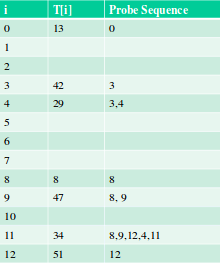
\includegraphics[scale=0.35]{final.png}
\column{0.5\textwidth}
\vspace{-1cm}
{\tiny
\begin{itemize}
\item 8 - straight in position 8.
\item 42 - stright in position 3.
\item 29:
\begin{itemize}
\tiny
\item $29\%13 = 3$ - 3 is full,
\item $(3+1)\%13 = 4$ - inserted into 4.
\end{itemize}
\item 51 - straight into 12.
\item 47:
\begin{itemize}
\tiny
\item $47\%13 = 8$ - 8 is full,
\item $(8+1)\%13 = 9$ - inserted into 9.
\end{itemize}
\item 13 - straight into 0
\item 34:
\begin{itemize}
\tiny
\item $34\%13 = 8$ - 8 is full,
\item $(8+1)\%13 = 9$ - 9 is full,
\item $(9+3)\%13 = 12$ - 12 is full,
\item $(12+5)\%13 = 4$ - 4 is full,
\item $(4+7)\%13 = 11$ - inserted into 11
\end{itemize}
\end{itemize}
}
\end{columns}
\end{frame}
%---------------------------------------------------------------
\defverbatim[colored]\dh{
\begin{lstlisting}[style = custom]
int i = h(k);
while (T[i].key != emptyKey) {
	i += r-(k%r)%size;
}
T[i].key = k;
T[i].data = d;
\end{lstlisting}
}
\subsection{Double Hashing}
\begin{frame}
\frametitle{Double Hashing}
\begin{itemize}
\item Use another hash functionas the increment function.
\item E.g. $h_2(k) = r - (k\%r)$
\item Same increment is added each stage, but the increment is different for different keys.
\end{itemize}
\dh
\end{frame}
%----------------------------------------------------------------
\subsubsection{Example}
\begin{frame}
\frametitle{Example}
\begin{itemize}
\item $h(k) = k\%13$
\item $h_2(k) = 5-(k\%5)$
\item Insert 8,42,29,50,47,13,26
\end{itemize}
\begin{columns}[c]
\column{0.5\textwidth}
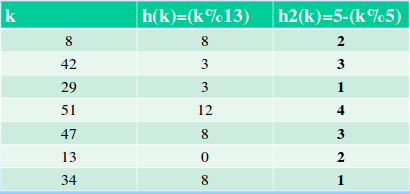
\includegraphics[scale=0.3]{hs.png}\\
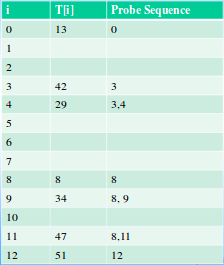
\includegraphics[scale=0.4]{finaldh.png}
\column{0.5\textwidth}
\begin{itemize}
\tiny
\item 8 - straight into 8
\item 42 - straight into 3
\item 29:
\begin{itemize}
\tiny
\item $29\%13 = 3$ - 3 is full,
\item $(3+1)\%13 = 4$ - inserted into 4
\end{itemize}
\item 51 - straight into 12
\item 47:
\begin{itemize}
\tiny
\item $47\%13 = 8$ - 8 is full,
\item $(8+3)\%13 = 11$ - inserted into 11
\end{itemize}
\item 13 - inserted into 0
\item 34:
\begin{itemize}
\tiny
\item $34\%13 = 8$ - 8 is full,
\item $(8+1) = 9$ - insert into 9. 
\end{itemize}
\end{itemize}
\end{columns}
\end{frame}
%---------------------------------------------------------------
\subsection{Rehashing}
\begin{frame}
\frametitle{Rehashing}
\begin{itemize}
\item If $T$ gets too full, the running time for operations increases and for hashing with quadratic probing, inserts may fail.
\item A solution is to build another hash table, $T2$, approximately the size of $T$ e.g. double size and then increase to the next prime number.
\item $T$ is then scanned and each (non-deleted) key from $T$ is inserted into $T2$
\end{itemize}
\end{frame}
%----------------------------------------------------------------
\begin{frame} 
\Huge{\centerline{The End}}
\end{frame}

\end{document}